% ====chapter=====
\myChapter{Approche d'ingénierie proposée pour la génération d'applications web pilotées par BPMN}{}
\label{chap:framework-prooweb}
\myMiniToc{mysection}{Sommaire}

\mySection{Introduction}{}

Ce chapitre présente l'approche proposée pour générer une application web métier à partir d'un modèle BPMN complété par une spécification applicative. Cette approche est concrétisée dans ProOWeb, le framework développé dans ce travail.

L'objectif est de montrer comment l'approche conserve la traçabilité entre le processus et le code généré, tout en laissant au développeur la possibilité d'adapter l'application. Le chapitre présente successivement la vue d'ensemble, l'architecture, la spécification d'entrée, les transformations et les mécanismes de préservation du code personnalisé.
\mySection{Vue d'ensemble de l'approche}{}
\label{sec:chap3-vue-ensemble}

\subsection{Problème traité et principe général}

L’approche proposée vise à générer une application web métier à partir
d’un processus métier modélisé. ProOWeb doit fournir un socle applicatif que le
développeur peut tester, adapter, versionner et maintenir.

Le choix de BPMN comme modèle d’entrée se justifie par sa capacité à représenter
les activités, événements, passerelles et flux d’un processus métier
. Toutefois, BPMN ne décrit pas toujours les informations
nécessaires à la génération d’une application web, telles que les formulaires, les
droits d’accès, la persistance ou les règles d’affectation. Pour cette raison, ProOWeb repose sur
un double modèle d’entrée : le fichier BPMN décrit le déroulement du processus,
tandis que la spécification \textit{spec-v1} fournit les détails applicatifs
nécessaires.

Le fonctionnement général suit quatre étapes : analyser le modèle BPMN, lire la
spécification \textit{spec-v1}, construire un modèle applicatif intermédiaire,
puis générer les artefacts liés à l’interface, à la logique métier, aux données, à
la sécurité et au suivi du processus.

\subsection{Positionnement dans le cycle MDA}

La Model-Driven Architecture fournit un cadre pertinent pour comprendre la progression proposée. ProOWeb ne reprend pas ce cadre comme une classification abstraite ; il l'utilise pour clarifier les responsabilités de chaque niveau de la chaîne de génération.

%Au niveau PIM, le processus est décrit sans dépendance directe à une technologie particulière d'interface, de serveur, de persistance ou de déploiement. Le BPMN représente le comportement métier, tandis que \textit{spec-v1} complète la conception applicative sans encore imposer la forme exacte des structures logicielles ou des composants d'interface. La spécification reste donc proche des préoccupations métier et applicatives : qui peut démarrer une instance, qui peut traiter une tâche, quelles données sont consultées, quelles sorties sont produites et quels rôles peuvent voir les informations.

%Au niveau PSM, ProOWeb construit des contrats intermédiaires : \textit{runtime contract}, \textit{data contract}, catalogues d'interface, catalogues de formulaires et registres de processus. Ces contrats sont plus proches de l'application cible. Ils indiquent les transitions, les rôles, les stratégies d'affectation, les sources de données, les mappings de sortie et les éléments à exposer à l'interface utilisateur. Ils ne sont pas encore du code source, mais ils rendent les informations suffisamment précises pour que les gabarits puissent produire des artefacts cohérents.

%Au niveau code, les transformations modèle-à-texte matérialisent les décisions précédentes. Une activité manuelle devient une tâche accessible dans l'interface, un point d'accès applicatif, une règle d'autorisation et une transition de runtime. Une donnée partagée devient une structure persistante, un espace de stockage et un champ exploitable par les formulaires. Une règle de visibilité devient un filtrage côté service applicatif et une adaptation côté interface.

\begin{table}[H]
\centering
\caption{Positionnement de ProOWeb dans le cycle MDA}
\label{tab:chap3-positionnement-mda}
\begin{tabularx}{\textwidth}{p{3.2cm}p{5.2cm}X}
\toprule
\textbf{Niveau} & \textbf{Contenu dans ProOWeb} & \textbf{Rôle dans la génération} \\
\midrule
PIM & BPMN et spécification \textit{spec-v1} & Décrire le workflow, les rôles, les entrées, les sorties, la visibilité et les données sans dépendre directement du code cible. \\
PSM & Contrats intermédiaires, catalogues et registres & Stabiliser les informations dans une forme exploitable par les générateurs d'interface, de logique applicative et de gestion des données. \\
Code & Projet applicatif comprenant interface, logique métier, données, sécurité et configuration & Produire une application web métier complète, fonctionnelle, exécutable, versionnable et personnalisable. \\
\bottomrule
\end{tabularx}
\end{table}

%Ce positionnement permet de réduire un risque classique des générateurs : concentrer trop de logique dans les templates. Dans ProOWeb, les gabarits ne doivent pas deviner les règles métier. Ils traduisent des décisions déjà validées dans le modèle pivot. Cette séparation améliore la traçabilité et facilite les tests de la chaîne de génération.

\subsection{Contribution méthodologique de l'approche}

La contribution de ce travail se situe à l'intersection de trois préoccupations. La première est la modélisation du processus. Le BPMN reste la référence du workflow et permet de maintenir une continuité avec les pratiques de modélisation métier. La deuxième est la génération d'une application web métier. Le framework ProOWeb ne se limite pas à produire des écrans ou des services isolés ; il organise un projet cible avec ses modules fonctionnels et techniques. La troisième est la maintenance du code généré. La régénération est traitée comme une opération contrôlée, accompagnée par un manifeste, des sauvegardes, des rapports et des mécanismes d'extension.

ProOWeb vise donc à produire un résultat directement exploitable par une équipe de développement et par les acteurs métier : une application web métier fonctionnelle, générée à partir du processus, mais ouverte à l'adaptation.

\mySection{Architecture globale du framework proposé}{}
\label{sec:chap3-architecture}

L'architecture de ProOWeb est organisée autour de quatre parties complémentaires. La première regroupe les modèles d'entrée. La deuxième correspond au noyau de génération du framework. La troisième représente l'application web produite. La quatrième concerne l'exploitation et l'évolution de cette application. Cette lecture par blocs permet de distinguer clairement ce qui est fourni par le concepteur, ce qui est traité par ProOWeb, ce qui est généré et ce qui est utilisé ensuite par les acteurs du système.

\begin{figure}[H]
\centering
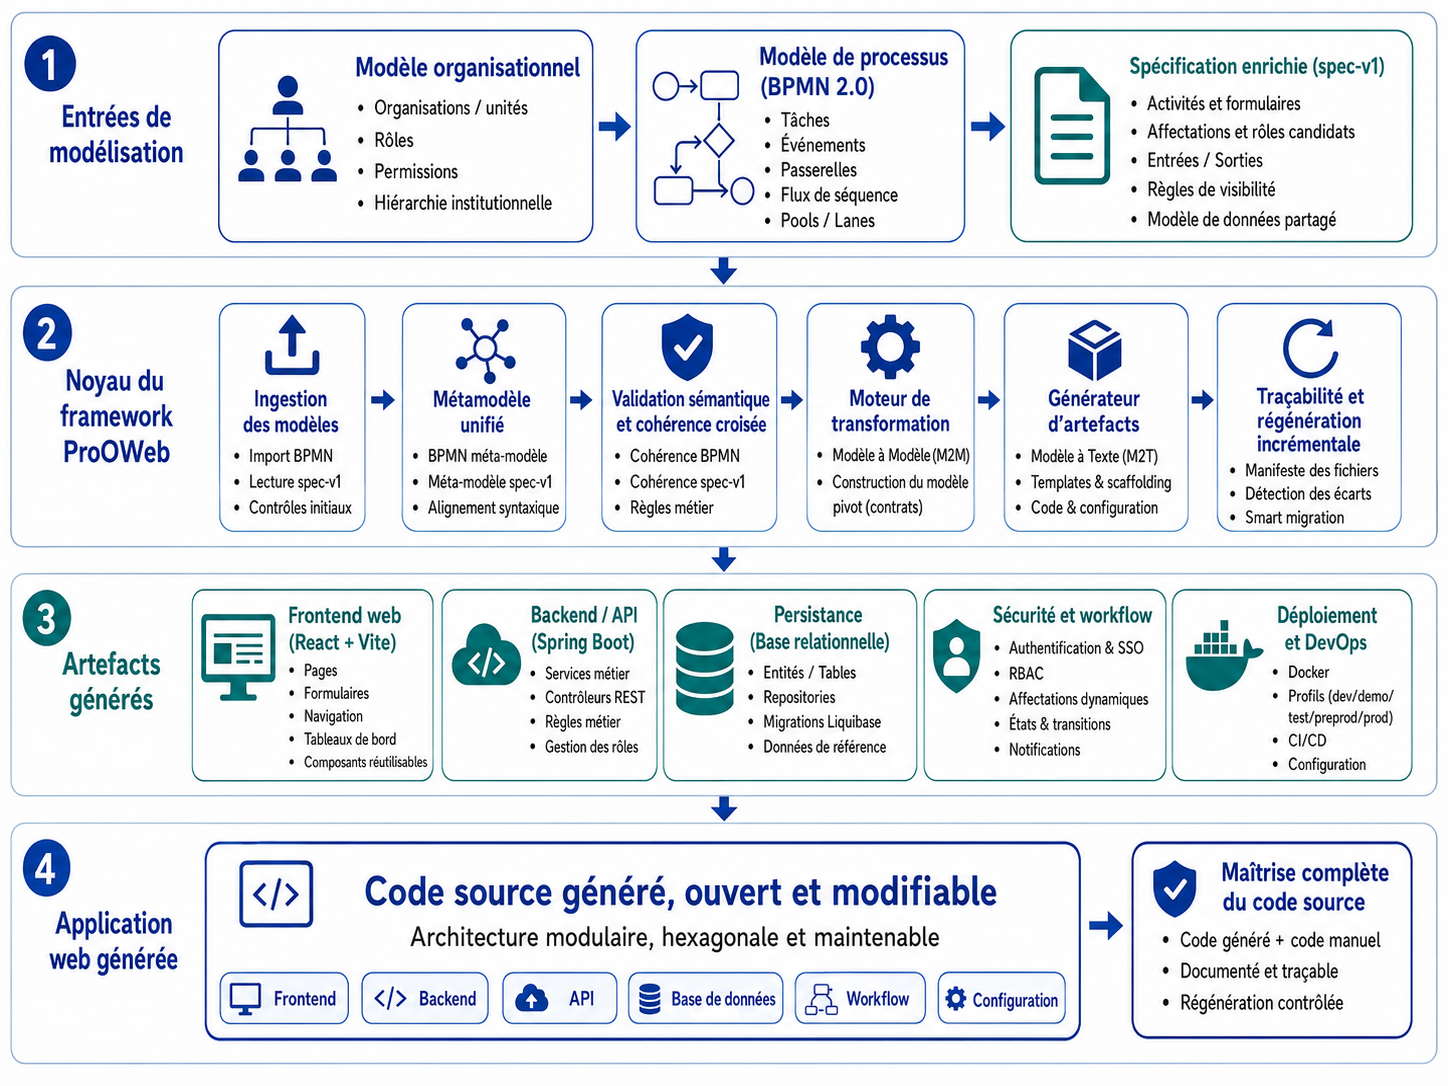
\includegraphics[width=0.82\textwidth]{Chap3/images/architecture_ProOWeb1.png}
\caption{Architecture générale de ProOWeb}
\label{fig:chap3-architecture-prooweb}
\end{figure}

\subsection{Modèles d'entrée de ProOWeb}

Le premier bloc de l’architecture constitue le point de départ de la génération.
Il regroupe le modèle BPMN, la spécification \textit{spec-v1}, les informations
organisationnelles et la configuration du projet cible. Le modèle BPMN décrit le
déroulement du processus à travers les activités, événements, passerelles et flux,
tandis que la spécification \textit{spec-v1} apporte les éléments nécessaires à
l’application, notamment les rôles, les données, les règles d’affectation, de
stockage et de visibilité. Les informations organisationnelles relient les tâches
aux acteurs concernés, alors que la configuration précise les options générales
du projet à générer. Ce bloc joue ainsi le rôle de source de vérité : ProOWeb y
lit, valide et transforme les informations métier afin de préserver la traçabilité
entre le modèle initial et le code produit.

\subsection{Noyau de génération du framework}

Ce bloc permet de transformer les modèles d’entrée en artefacts générables à travers plusieurs traitements : ingestion du
BPMN, enrichissement par la spécification \textit{spec-v1}, validation croisée,
construction du modèle pivot et génération des fichiers applicatifs. L’ingestion
extrait les activités, événements, passerelles et flux du processus, puis
l’enrichissement associe à chaque activité les rôles, données, règles de
visibilité et comportements définis dans la spécification. La validation vérifie
ensuite la cohérence entre le BPMN et \textit{spec-v1}, afin d’éviter une
application générée fonctionnellement incorrecte. Après cette étape, ProOWeb
construit un modèle pivot composé de contrats intermédiaires, tels que le
\textit{runtime contract}, le \textit{data contract}, les catalogues d’interface
et le registre des processus. Ces contrats structurent les transformations
modèle-à-modèle et modèle-à-texte nécessaires à la production du code source.

\subsection{Application web générée}

Ici, il ne s’agit pas d’un simple assemblage de fragments, mais d’un projet web métier structuré,
exécutable et exploitable par les acteurs concernés. L’application générée
comprend les vues de traitement, les listes de tâches, les formulaires, les
interfaces de suivi et les espaces de supervision. Elle intègre également les
services nécessaires au démarrage d’un processus, à l’exécution des activités, à
la gestion des transitions, à la persistance des données et au contrôle des
droits d’accès. Les données peuvent être rattachées à une instance de processus
ou conservées comme informations partagées, selon les règles définies dans
\textit{spec-v1}. Ainsi, ProOWeb produit une base applicative complète, reliant
interface, logique métier, sécurité, données, exécution du workflow et
configuration du projet cible.

\subsection{Exploitation et évolution de l'application}

Après la génération, l’application est utilisée par les acteurs métier
pour exécuter les tâches, par les superviseurs pour suivre les instances, par les
administrateurs pour gérer les paramètres et par les développeurs pour adapter le
code lorsque des besoins spécifiques apparaissent. Cette dimension évolutive est
essentielle, car un processus, une règle d’affectation, un champ ou une interface
peuvent être modifiés au cours du temps. ProOWeb prend donc en compte la
régénération à travers le suivi des fichiers produits, la détection des
modifications manuelles, la création de sauvegardes et la production de rapports
de migration. L’architecture forme ainsi une boucle itérative reliant les modèles,
le code généré et les adaptations réalisées.

%\begin{table}[H]
%\centering
%\small
%\caption{Rôle des principales parties de l'architecture ProOWeb}
%\label{tab:chap3-parties-architecture}
%\begin{tabular}{p{3.5cm}p{4.8cm}p{5.4cm}}
%\hline
%\textbf{Partie de l'architecture} & \textbf{Contenu principal} & \textbf{Rôle dans l'approche} \\
%\hline
%Modèles d'entrée & BPMN, \textit{spec-v1}, rôles, données et configuration & Fournir les informations métier et applicatives nécessaires à la génération. \\
%Noyau ProOWeb & Ingestion, validation, modèle pivot, transformations et templates & Transformer les modèles en contrats puis en artefacts logiciels. \\
%Application générée & Interface, logique applicative, données métier, sécurité, exécution du processus et suivi & Produire une application web métier complète et fonctionnelle. \\
%Exploitation et évolution & Utilisateurs, supervision, manifeste, sauvegardes et migration & Permettre l'utilisation, l'adaptation et la régénération contrôlée de l'application. \\
%\hline
%\end{tabular}
%\end{table}

\mySection{Modèle d'entrée enrichi : spécification spec-v1}{}
\label{sec:chap3-spec}

%\subsection{Rôle de la spécification enrichie}

La spécification \textit{spec-v1} constitue le complément applicatif du modèle BPMN. Elle rend explicites les informations nécessaires à la génération d'une application web métier. Son rôle est donc de décrire ce que BPMN ne porte pas naturellement : rôles autorisés, supervision, stratégie d'affectation, données d'entrée, sorties, règles de visibilité, stockage et comportement des activités automatiques.

%Cette séparation repose sur une idée simple. Le BPMN doit rester lisible comme modèle de processus, tandis que la spécification doit contenir les informations nécessaires à l'application. Si toutes les règles applicatives étaient injectées dans le diagramme, le modèle deviendrait difficile à lire. Si elles étaient placées uniquement dans le code, la traçabilité entre processus et application serait perdue. \textit{Spec-v1} joue donc un rôle de médiation entre le modèle métier et le projet généré.

\subsection{Structure générale de spec-v1}

La structure de \textit{spec-v1} est organisée autour de blocs fonctionnels. Le bloc de démarrage indique les rôles autorisés à lancer une instance et les activités initiales. Le bloc de supervision précise les rôles capables de suivre ou d'administrer le processus. Le bloc des activités décrit chaque étape BPMN à enrichir. Le bloc des données partagées définit les entités persistantes et leurs champs. Cette organisation rend la spécification lisible et vérifiable.

\begin{lstlisting}[caption={Structure simplifiée de la spécification spec-v1},label={lst:chap3-structure-specv1}]
{
  "processId": "processus_demande",
  "schemaVersion": 1,
  "start": {
    "allowedRoles": ["DEMANDEUR"],
    "startActivities": ["saisir_demande"]
  },
  "monitoring": {
    "supervisorRoles": ["SUPERVISEUR", "ADMINISTRATEUR"]
  },
  "activities": {
    "saisir_demande": {
      "activityType": "MANUAL",
      "assignment": {},
      "input": {},
      "output": {},
      "visibility": {}
    }
  },
  "sharedData": {
    "entities": []
  }
}
\end{lstlisting}

Pour que cette spécification puisse être exploitée par un générateur, sa structure ne doit pas rester implicite. Dans ProOWeb, \textit{spec-v1} est considérée comme un contrat d'entrée : certains champs sont obligatoires, d'autres sont optionnels, et plusieurs valeurs appartiennent à des listes contrôlées. Cette formalisation évite que deux utilisateurs décrivent le même besoin avec des formes différentes et permet au générateur de produire des diagnostics précis avant la génération.

\begin{table}[H]
\centering
\caption{Définition formelle des principaux champs de la spécification \textit{spec-v1}}
\label{tab:chap3-definition-formelle-specv1}
\begin{tabularx}{\textwidth}{p{5.3cm}p{3.0cm}X}
\toprule
\textbf{Champ} & \textbf{Type attendu} & \textbf{Contrainte principale} \\
\midrule
\texttt{processId} & Chaîne & Identifiant stable du processus ; il doit correspondre au processus BPMN importé. \\
\texttt{schemaVersion} & Entier & Version du format de spécification ; pour ce travail, la valeur attendue est \texttt{1}. \\
\texttt{start.allowedRoles} & Liste de rôles & Chaque rôle doit appartenir au référentiel de rôles de l'application. \\
\texttt{activities} & Objet indexé & Chaque clé doit être l'identifiant d'une activité BPMN enrichie. \\
\texttt{activityType} & Enumération & Valeurs autorisées : \texttt{MANUAL} ou \texttt{AUTOMATIC}. \\
\texttt{assignment.candidateRoles} & Liste de rôles & Une tâche manuelle doit toujours avoir au moins un rôle capable de la traiter. \\
\bottomrule
\end{tabularx}
\end{table}

%Les types autorisés restent volontairement simples : chaînes, entiers, booléens, listes, objets structurés et énumérations. Les champs d'une entité partagée peuvent par exemple être typés en \texttt{string}, \texttt{number}, \texttt{boolean}, \texttt{date}, \texttt{datetime} ou \texttt{file}. La spécification utilise donc des valeurs contrôlées. Les types d'activités distinguent les tâches manuelles et automatiques, les stratégies d'affectation sont bornées par une liste connue, et les stratégies de stockage indiquent explicitement où les données produites doivent être conservées. Cette discipline limite les ambiguïtés et rend la génération plus déterministe.

\subsection{Métadonnées des activités}

Les métadonnées d'activité indiquent comment une étape BPMN doit être prise en charge dans l'application. Une activité manuelle est destinée à être traitée par un utilisateur. Elle doit donc préciser les rôles candidats, la stratégie d'affectation, les données visibles, les sorties attendues et les règles de complétion. Une activité automatique est exécutée par le système. Elle doit alors indiquer le gestionnaire à invoquer, son type, son mode de déclenchement et sa configuration.

\begin{lstlisting}[caption={Exemple d'activité enrichie dans spec-v1},label={lst:chap3-activite-enrichie}]
"valider_demande": {
  "activityType": "MANUAL",
  "assignment": {
    "candidateRoles": ["VALIDATEUR"],
    "mode": "CLAIM",
    "strategy": "ROLE_BASED"
  },
  "input": {
    "sources": ["PROCESS_CONTEXT", "PREVIOUS_ACTIVITY"]
  },
  "output": {
    "storage": "BOTH",
    "mappings": []
  },
  "visibility": {
    "activityViewerRoles": ["VALIDATEUR", "SUPERVISEUR"],
    "dataViewerRoles": ["VALIDATEUR"]
  }
}
\end{lstlisting}

Cet exemple montre le passage du processus vers l'application. L'identifiant \texttt{valider\_demande} renvoie à une activité BPMN. Les rôles candidats orientent l'affectation de la tâche. Les sources d'entrée indiquent les données disponibles pour le formulaire. La stratégie de stockage précise où seront conservées les sorties. Les règles de visibilité distinguent les acteurs qui peuvent voir l'activité de ceux qui peuvent accéder aux données.

\subsection{Affectation des tâches et sécurité}

L'affectation des tâches est un point central dans une application web métier. Une tâche doit être proposée aux bons utilisateurs, selon les responsabilités prévues par l'organisation. Dans ProOWeb, cette dimension est décrite par les rôles candidats, le mode d'affectation et la stratégie d'assignation.

%Plusieurs stratégies peuvent être représentées. Une stratégie de file par rôle rend la tâche disponible aux utilisateurs possédant les rôles candidats. Une stratégie supervisée oriente la tâche vers un superviseur. Une stratégie hiérarchique peut remonter vers des responsables lorsque le premier niveau n'est pas disponible. Ces choix ne relèvent pas seulement de l'ergonomie. Ils influencent la sécurité de l'application, car ils déterminent qui peut voir, réclamer, traiter ou déléguer une tâche.

\begin{table}[H]
\centering
\caption{Exemples de stratégies d'affectation}
\label{tab:chap3-strategies-affectation}
\begin{tabularx}{\textwidth}{p{6.2cm}X}
\toprule
\textbf{Stratégie} & \textbf{Interprétation dans ProOWeb} \\
\midrule
\texttt{ROLE\_QUEUE} & La tâche est visible dans une file associée aux rôles candidats. \\
\texttt{ROLE\_BASED} & La tâche est attribuée ou réclamée selon les rôles déclarés dans la spécification. \\
\texttt{SUPERVISOR\_ONLY} & La tâche est réservée aux rôles de supervision. \\
\texttt{SUPERVISOR\_THEN\_ANCESTORS} & La tâche peut être escaladée dans une chaîne hiérarchique lorsque la règle locale ne suffit pas. \\
\bottomrule
\end{tabularx}
\end{table}

\subsection{Entrées, sorties et données partagées}

Une application web métier ne se contente pas d'enchaîner des tâches. Elle manipule des informations. ProOWeb distingue les données propres à une instance (décrivant l'état d'une exécution particulière) et les données partagées (représentant des informations métier réutilisables, persistées et consultables au-delà d'une instance).

Les entrées d'une activité peuvent provenir du contexte du processus, d'une activité précédente, d'une donnée partagée ou d'une source externe. Les sorties peuvent être stockées dans l'instance, dans les données partagées ou dans les deux espaces.

Le bloc \texttt{sharedData} définit les entités partagées. Ces entités peuvent ensuite être projetées vers des classes de domaine, des repositories, des migrations de schéma et des métadonnées de formulaires. Lorsque les mappings de sortie indiquent qu'une activité produit une donnée partagée, ProOWeb peut établir le lien entre la tâche, le champ produit et la structure persistante cible.

\begin{table}[H]
\centering
\caption{Correspondance entre informations d'entrée et application générée}
\label{tab:chap3-correspondance-entree-generation}
\begin{tabularx}{\textwidth}{p{3.6cm}p{4.5cm}X}
\toprule
\textbf{Information d'entrée} & \textbf{Projection intermédiaire} & \textbf{Artefact généré} \\
\midrule
Activité BPMN & Activité du \textit{runtime contract} & Tâche runtime, vue de traitement et action de complétion. \\
Flux BPMN & Transitions et liens entrants/sortants & Logique d'orchestration et progression d'instance. \\
Rôles candidats & Politique d'affectation & Liste de tâches, assignation et contrôle d'accès. \\
Sources d'entrée & Lignage des données & Pré-remplissage de formulaires et résolution de contexte. \\
Mappings de sortie & Stratégie de stockage & Mise à jour de l'instance, des données partagées ou des deux. \\
Règles de visibilité & Droits de lecture activité/donnée & Filtrage applicatif et adaptation de l'interface. \\
Données partagées & Entités, champs et relations & Modèles persistants, migrations et métadonnées. \\
\bottomrule
\end{tabularx}
\end{table}


\subsection{Règles de visibilité}

La visibilité ne se réduit pas à l'affectation. Un utilisateur peut être autorisé à consulter une instance sans être autorisé à traiter la tâche courante. De même, un superviseur peut voir l'état d'un processus sans accéder à toutes les données sensibles produites par les activités. ProOWeb distingue donc la visibilité des activités et la visibilité des données.

Cette distinction permet de générer des filtres plus fins côté services applicatifs et des interfaces plus adaptées côté utilisateur. Les services applicatifs peuvent masquer certaines tâches ou certaines données selon le rôle de l'utilisateur. Les composants d'interface peuvent également adapter les informations affichées sans exposer inutilement des données sensibles.

\mySection{Règles de transformation et génération de l'application web}{}
\label{sec:chap3-transformations}

Les règles de transformation déterminent la manière dont le double modèle d'entrée devient une application web métier. Dans ProOWeb, la transformation suit deux moments principaux. La transformation modèle-à-modèle construit le modèle applicatif intermédiaire. La transformation modèle-à-texte produit les fichiers du projet cible. Ce découpage permet de vérifier les contrats avant l'écriture du code.

\subsection{Validation avant génération}

La validation est une étape indispensable. Une erreur dans les modèles d'entrée peut se propager dans plusieurs fichiers générés : point d'accès applicatif, composant d'interface, transition, structure de données ou règle de sécurité. Le framework doit donc refuser ou signaler les situations ambiguës avant de produire le projet cible.

Les contrôles portent sur quatre dimensions. La dimension structurelle vérifie que les activités enrichies existent dans le BPMN et que les transitions forment un graphe exploitable. La dimension applicative vérifie que les activités manuelles disposent d'informations suffisantes pour être traitées par un utilisateur. La dimension données vérifie que les entrées, sorties et mappings référencent des structures connues. La dimension sécurité vérifie la cohérence des rôles utilisés pour l'exécution, la supervision et la visibilité.

\begin{table}[H]
\centering
\caption{Exemples de contrôles réalisés avant génération}
\label{tab:chap3-controles-generation}
\begin{tabularx}{\textwidth}{p{3.8cm}p{5.2cm}X}
\toprule
\textbf{Dimension} & \textbf{Règle contrôlée} & \textbf{Risque évité} \\
\midrule
Structure BPMN & Toute activité enrichie doit exister dans le modèle BPMN. & Artefacts sans activité correspondante. \\
Sécurité & Une tâche manuelle doit posséder au moins un rôle candidat. & Tâche exposée sans responsabilité claire. \\
Données & Un mapping de sortie doit cibler une donnée connue. & Perte ou mauvaise persistance des données. \\
Workflow & Une transition générée doit correspondre à un chemin possible. & Divergence entre modèle et runtime. \\
Interface & Les champs affichés doivent provenir d'une source déclarée. & Formulaire incohérent avec le contexte. \\
\bottomrule
\end{tabularx}
\end{table}

Ces contrôles doivent produire des diagnostics compréhensibles. L'utilisateur du framework doit pouvoir identifier l'activité, la règle ou la donnée responsable de l'erreur.

\subsection{Transformation modèle-à-modèle}

La transformation modèle-à-modèle prend en entrée le BPMN et \textit{spec-v1}. Elle commence par normaliser les activités. Chaque activité reçoit un type, des rôles candidats, une politique d'affectation, des entrées, des sorties et une visibilité. Les activités automatiques reçoivent en plus un gestionnaire, un type de tâche automatique, un mode de déclenchement et une configuration.

À partir du BPMN, ProOWeb détermine les transitions entre activités, les liens entrants et les liens sortants. Les activités de départ peuvent être configurées explicitement ou inférées à partir du graphe. Cette étape permet au runtime de savoir comment démarrer une instance et comment la faire progresser.

Les mappings d'entrée et de sortie sont parcourus afin de relier les activités, les champs produits, les entités partagées et les sources utilisées. Cette représentation permet de comprendre comment une information circule dans le processus et comment elle se matérialise dans l'application.

\textbf{Construction du modèle applicatif intermédiaire}

Le modèle applicatif intermédiaire regroupe uniquement les informations nécessaires à la génération : déroulement du processus, rôles, données, formulaires et traces des artefacts produits. Il sert de contrat entre l'analyse du BPMN, l'enrichissement \textit{spec-v1} et les gabarits de génération.

\begin{table}[H]
\centering
\caption{Structures principales du modèle pivot ProOWeb}
\label{tab:chap3-structures-modele-pivot}
\begin{tabularx}{\textwidth}{p{4.1cm}X}
\toprule
\textbf{Structure conservée} & \textbf{Utilité dans ProOWeb} \\
\midrule
\texttt{ProcessModel} & Garde la référence au processus BPMN, à ses activités et à ses transitions. \\
\texttt{ActivityModel} & Transforme chaque activité BPMN enrichie en unité exploitable par l'application. \\
\texttt{RolePolicy} & Regroupe les rôles, règles d'affectation, droits d'accès et restrictions de visibilité. \\
\texttt{FormModel} & Décrit les champs affichés, les sorties produites et les validations des formulaires. \\
\texttt{RuntimeContract} & Fournit au moteur d'exécution les états, transitions et actions disponibles. \\
\texttt{DataContract} & Prépare les entités, champs, mappings et règles de stockage des données. \\
\texttt{ArtifactTrace} & Relie les éléments du modèle aux fichiers générés afin de contrôler les régénérations. \\
\bottomrule
\end{tabularx}
\end{table}

%Cette décomposition permet de maîtriser la complexité. Une activité manuelle touche plusieurs vues : elle appartient au workflow, elle est exécutée par certains rôles, elle manipule des données, elle apparaît dans une interface et elle déclenche un cas d'utilisation. Le modèle pivot regroupe ces informations sans les confondre. Les gabarits d'interface peuvent utiliser principalement la vue interface, tandis que les gabarits applicatifs utilisent la vue processus, la vue sécurité et la vue données.

%La construction du modèle pivot doit aussi conserver la traçabilité. Chaque élément généré doit pouvoir être relié à une activité, une entité ou une règle de la spécification. Cette traçabilité facilite la maintenance. Lorsqu'un changement intervient dans le BPMN ou dans \textit{spec-v1}, le framework peut identifier les artefacts concernés et limiter l'impact de la régénération.

\subsection{Transformation modèle-à-texte}

La transformation modèle-à-texte produit les fichiers de l'application. Les gabarits reçoivent les éléments du modèle pivot et les projettent dans les artefacts cibles. Le passage vers le texte transforme alors des structures abstraites en vues, composants, services, règles d'accès, structures de données et fichiers de configuration.

La qualité de cette transformation dépend de la précision des gabarits. Un gabarit ne doit pas contenir des décisions métier cachées. Il doit traduire les décisions déjà prises dans le modèle pivot. Par exemple, si une activité est réservée au rôle \texttt{VALIDATEUR}, le gabarit d'accès applicatif doit utiliser cette information pour produire le contrôle d'accès correspondant. Si une entité possède une contrainte de non-nullité, le gabarit de persistance et le formulaire associé doivent en tenir compte.

Le moteur M2T doit également conserver une organisation déterministe. À modèle identique, il doit produire la même structure de projet, les mêmes noms d'artefacts et les mêmes emplacements de fichiers. Cette propriété facilite la comparaison entre deux générations, l'identification des changements et la synchronisation avec un gestionnaire de versions.

\subsection{Exemple de traçabilité de bout en bout}

La traçabilité est illustrée ici sur l'activité BPMN \texttt{valider\_demande}. L'intérêt n'est pas de détailler séparément chaque couche technique, mais de montrer comment une intention métier reste reconnaissable jusqu'aux éléments produits par ProOWeb.

\begin{table}[H]
\centering
\caption{Exemple de traçabilité d'une activité BPMN vers les artefacts générés}
\label{tab:chap3-exemple-tracabilite}
\begin{tabularx}{\textwidth}{p{3.8cm}X}
\toprule
\textbf{Niveau suivi} & \textbf{Interprétation dans ProOWeb} \\
\midrule
BPMN & La tâche \texttt{valider\_demande} donne le point de passage métier et ses liens avec le reste du processus. \\
\textit{spec-v1} & L'activité reçoit les précisions absentes du diagramme : rôle autorisé, données utiles, sorties attendues et visibilité. \\
Modèle pivot & ProOWeb rassemble ces informations dans une représentation stable, utilisable par les règles de génération. \\
Artefacts générés & Les fichiers produits matérialisent la même activité : écran de traitement, action de validation, contrôle d'accès et mise à jour des données. \\
Manifeste & Les fichiers rattachés à cette activité restent identifiables afin de maîtriser les futures régénérations. \\
\bottomrule
\end{tabularx}
\end{table}

%Cet exemple montre que la traçabilité ne se limite pas à un lien documentaire entre le BPMN et le code. Elle sert à expliquer pourquoi un artefact existe, de quelle activité il provient et quelle partie du contrat il matérialise. Elle sert aussi lors de l'évolution du processus : si \texttt{valider\_demande} change de rôle, de formulaire ou de sortie, ProOWeb peut identifier les contrats et les fichiers concernés par la nouvelle génération.

\subsection{Règles de projection vers les artefacts}

Les règles de projection définissent comment chaque élément du modèle pivot est traduit dans l'application cible. Elles ne sont pas de simples conventions de nommage. Elles indiquent la couche de destination et la responsabilité de l'artefact produit.

\begin{table}[H]
\centering
\caption{Exemples de règles de projection vers l'application générée}
\label{tab:chap3-projection-m2t}
\begin{tabularx}{\textwidth}{p{3.8cm}p{4.8cm}X}
\toprule
\textbf{Élément du modèle pivot} & \textbf{Artefact généré} & \textbf{Couche cible} \\
\midrule
Activité manuelle & Formulaire, page d'activité, structure d'entrée & Interface utilisateur et couche applicative. \\
Activité automatique & Opération système ou service applicatif & Couche applicative. \\
Rôle candidat & Règle d'accès et filtre de tâche & Sécurité, services applicatifs et interface. \\
Transition du workflow & Méthode de progression et changement d'état & Runtime du processus. \\
Entité partagée & Structure métier, stockage, migration & Domaine et persistance. \\
Mapping de sortie & Service de sauvegarde et projection cible & Application et persistance. \\
\bottomrule
\end{tabularx}
\end{table}

Cette projection maintient la cohérence entre le modèle et le projet produit. Le générateur ne crée pas seulement des fichiers ; il garde le lien entre chaque élément généré et le besoin métier qui l'a rendu nécessaire. Ce lien rend le code plus compréhensible lorsqu'il faut l'adapter ou le régénérer.

%Dans le projet cible, ProOWeb ne cherche pas à multiplier les fichiers pour chaque couche technique. Les artefacts générés sont regroupés autour des besoins concrets de l'application : exécuter le processus, faire traiter les tâches, conserver les données, contrôler les accès et suivre les fichiers produits.

\begin{table}[H]
\centering
\caption{Inventaire des artefacts générés par ProOWeb}
\label{tab:chap3-inventaire-artefacts-generes}
\begin{tabularx}{\textwidth}{p{3.8cm}X}
\toprule
\textbf{Besoin couvert} & \textbf{Rôle dans l'application produite} \\
\midrule
Exécuter le processus & Démarrer une instance, proposer les tâches, appliquer les transitions et enregistrer l'avancement. \\
Traiter les activités & Donner aux acteurs les vues, formulaires et actions nécessaires pour accomplir leurs tâches. \\
Conserver les informations & Garder les données de l'instance, les données partagées et l'historique des actions importantes. \\
Contrôler les accès & Appliquer les rôles candidats, les règles de visibilité et les restrictions liées à chaque activité. \\
Suivre la génération & Identifier les fichiers produits, signaler les changements et protéger les adaptations manuelles. \\
\bottomrule
\end{tabularx}
\end{table}

%\subsection{Algorithme général de génération}

%L'algorithme suivant résume le déroulement logique de ProOWeb. Il ne représente pas toutes les instructions internes, mais il met en évidence les étapes nécessaires pour passer du double modèle d'entrée à une application web métier générée.

%\begin{lstlisting}[caption={Algorithme général de génération d'une application ProOWeb},label={lst:chap3-algorithme-generation}]
%Algorithme GenererApplicationWebPilotee
%Entrees :
  %modeleBpmn
  %specificationSpecV1
  %configurationProjet
%Sortie :
  %applicationWebGeneree

%Debut
  %workflow <- analyserModeleBpmn(modeleBpmn)
  %enrichissements <- lireSpecification(specificationSpecV1)

  %verifierCorrespondance(workflow, enrichissements)
  %verifierReglesApplicatives(enrichissements)

  %modelePivot <- construireModeleApplicatif(workflow, enrichissements)
  %verifierCoherence(modelePivot)

  %genererContratExecution(modelePivot)
  %genererContratDonnees(modelePivot)
  %genererCataloguesInterface(modelePivot)

  %preparerStructureProjet(configurationProjet)
  %genererLogiqueApplicative(modelePivot)
  %genererInterfaceUtilisateur(modelePivot)
  %genererPersistance(modelePivot)
  %genererConfigurationEtDeploiement(modelePivot)

  %mettreAJourManifeste()
  %produireRapportGeneration()
  %retourner applicationWebGeneree
%Fin
%\end{lstlisting}

%Cet algorithme met en évidence la place de la validation et des contrats. La génération n'intervient qu'après la normalisation du modèle et la construction du modèle pivot. Cette organisation rend le résultat plus fiable qu'une approche où les fichiers seraient écrits directement depuis le diagramme.

\mySection{Préservation du code personnalisé et synchronisation}{}
\label{sec:chap3-preservation}

Une difficulté importante de la génération d'application concerne l'évolution du projet après une première génération. Dans un contexte réel, les développeurs ajoutent des règles particulières, adaptent les interfaces, complètent des services ou intègrent des dépendances spécifiques. Si chaque nouvelle génération écrase ces modifications, le framework devient difficile à utiliser. ProOWeb traite donc la régénération comme une opération d'ingénierie, et non comme un simple remplacement de fichiers.

Cette préoccupation est bien identifiée dans les travaux sur la cohabitation entre code généré et code écrit à la main. Greifenberg et al. comparent plusieurs mécanismes d'intégration et montrent que le choix d'une stratégie influence directement la maintenabilité des systèmes générés \cite{greifenberg2015}.

\subsection{Problème de la régénération}

La régénération apparaît lorsqu'un processus évolue, lorsqu'une activité est ajoutée, lorsqu'une règle de données change. Elle est nécessaire pour maintenir l'application alignée sur les modèles. Elle est également risquée, car elle peut remplacer des fichiers modifiés par les développeurs.

Le problème ne se limite pas à la perte de code. Une régénération non contrôlée peut produire des conflits de fichiers, des incohérences entre la partie applicative et l'interface, la disparition de règles spécifiques, un changement non documenté dans la sécurité ou une rupture des tests. ProOWeb distingue donc les fichiers gérés par le générateur et les fichiers non gérés. Les fichiers gérés sont suivis dans le manifeste \texttt{.prooweb-managed.json}. Les fichiers non gérés restent hors du contrôle du générateur.

\subsection{Manifeste et contrat de propriété}

Le manifeste \texttt{.prooweb-managed.json} décrit les fichiers produits par ProOWeb. Pour chaque fichier, il peut conserver le chemin, la catégorie, les propriétaires logiques et une empreinte. Cette information permet de savoir si un fichier correspond toujours à la dernière version générée ou s'il a été modifié manuellement.

Ce manifeste définit un contrat de propriété. Un fichier généré et non modifié peut être remplacé lors d'une nouvelle génération. Un fichier généré mais modifié doit être traité avec prudence. Un fichier non géré ne doit pas être écrasé. Cette règle donne au développeur une garantie pratique : ProOWeb ne considère pas le projet cible comme un répertoire jetable.

\subsection{Préservation côté logique applicative}

Côté logique applicative, la préservation est particulièrement importante, car le code généré porte les API, la sécurité, la persistance et le runtime. ProOWeb limite le risque en produisant une architecture modulaire. Les éléments issus du modèle sont générés dans des couches précises, tandis que les adaptations locales peuvent être placées dans des modules ou points d'extension séparés.

Cette stratégie rejoint le principe du \textit{Generation Gap Pattern}, souvent utilisé pour séparer les classes générées des classes écrites manuellement \cite{greifenberg2015}. Le générateur peut produire un squelette ou une classe de base, tandis que le développeur ajoute un comportement spécifique dans une classe séparée. Lors d'une régénération, la partie contrôlée par ProOWeb peut évoluer sans supprimer les extensions manuelles.

La préservation ne doit toutefois pas servir à contourner le modèle. Si une modification concerne le workflow, les rôles, les données structurantes ou les règles de visibilité, elle devrait être reportée dans le BPMN ou dans \textit{spec-v1}. Les extensions manuelles doivent plutôt couvrir les détails d'intégration, les règles particulières ou les adaptations difficiles à généraliser.

\subsection{Préservation côté interface utilisateur}

Côté interface utilisateur, la personnalisation concerne souvent les libellés, les parcours utilisateur, les composants visuels, les contrôles d'ergonomie et certaines intégrations. ProOWeb génère les composants liés au processus, mais l'équipe doit pouvoir adapter l'expérience utilisateur sans perdre ses modifications lors d'un redéploiement.

La stratégie retenue repose sur la composition, la configuration et les overrides de templates. Les composants générés peuvent être encapsulés par des composants propres au projet. Les règles d'override déclarées peuvent remplacer, préfixer, suffixer ou modifier un bloc de contenu généré. Cette personnalisation est réappliquée lors des générations suivantes, ce qui réduit les modifications répétées directement dans les fichiers produits.

\subsection{Cycle de synchronisation itératif}

Le cycle de synchronisation décrit la manière dont ProOWeb accompagne les évolutions successives du modèle. Une première génération produit l'application de base. Les développeurs peuvent ensuite ajouter des extensions, adapter certains modules ou déclarer des overrides. Lorsque le BPMN ou \textit{spec-v1} évolue, ProOWeb reconstruit un snapshot de génération, compare l'état attendu avec l'état du projet, applique les règles de migration et produit un rapport.

Ce cycle transforme la génération en activité continue. L'application n'est pas simplement créée une fois ; elle peut être régénérée, migrée et adaptée. La synchronisation repose sur trois traces : le manifeste des fichiers gérés, les sauvegardes créées lors des conflits et les rapports de migration. Ces éléments permettent de comprendre ce qui a changé et de revenir sur une modification si nécessaire.

\begin{table}[H]
\centering
\caption{Mécanismes de préservation et de synchronisation dans ProOWeb}
\label{tab:chap3-preservation-synchronisation}
\begin{tabularx}{\textwidth}{p{3.8cm}p{5.0cm}X}
\toprule
\textbf{Mécanisme} & \textbf{Rôle} & \textbf{Effet attendu} \\
\midrule
Manifeste & Suivre les fichiers générés, leurs catégories et leurs empreintes. & Identifier les fichiers que ProOWeb peut gérer. \\
Migration contrôlée & Comparer l'état attendu et l'état réel du projet. & Éviter l'écrasement silencieux du code personnalisé. \\
Sauvegardes & Copier les fichiers conflictuels avant remplacement. & Permettre la récupération des adaptations manuelles. \\
Template overrides & Réappliquer des personnalisations déclarées. & Réduire les modifications manuelles répétées. \\
Rapports & Décrire les créations, mises à jour, conflits et sauvegardes. & Rendre l'évolution auditable et compréhensible. \\
\bottomrule
\end{tabularx}
\end{table}

\mySection{Conclusion}{}

Ce chapitre a présenté l'approche proposée et sa concrétisation dans le framework ProOWeb, depuis les modèles d'entrée jusqu'aux artefacts générés. Le BPMN décrit le déroulement du processus, \textit{spec-v1} apporte les informations applicatives nécessaires et le modèle pivot organise ces données avant la génération.

L'approche met l'accent sur deux points : maintenir la traçabilité entre le modèle et le code, puis permettre l'évolution contrôlée de l'application générée. Le chapitre suivant présente la mise en oeuvre technique de cette proposition et son application à un cas d'utilisation.
